% Options for packages loaded elsewhere
\PassOptionsToPackage{unicode}{hyperref}
\PassOptionsToPackage{hyphens}{url}
%
\documentclass[
]{article}
\usepackage{amsmath,amssymb}
\usepackage{lmodern}
\usepackage{iftex}
\ifPDFTeX
  \usepackage[T1]{fontenc}
  \usepackage[utf8]{inputenc}
  \usepackage{textcomp} % provide euro and other symbols
\else % if luatex or xetex
  \usepackage{unicode-math}
  \defaultfontfeatures{Scale=MatchLowercase}
  \defaultfontfeatures[\rmfamily]{Ligatures=TeX,Scale=1}
\fi
% Use upquote if available, for straight quotes in verbatim environments
\IfFileExists{upquote.sty}{\usepackage{upquote}}{}
\IfFileExists{microtype.sty}{% use microtype if available
  \usepackage[]{microtype}
  \UseMicrotypeSet[protrusion]{basicmath} % disable protrusion for tt fonts
}{}
\makeatletter
\@ifundefined{KOMAClassName}{% if non-KOMA class
  \IfFileExists{parskip.sty}{%
    \usepackage{parskip}
  }{% else
    \setlength{\parindent}{0pt}
    \setlength{\parskip}{6pt plus 2pt minus 1pt}}
}{% if KOMA class
  \KOMAoptions{parskip=half}}
\makeatother
\usepackage{xcolor}
\usepackage[margin=1in]{geometry}
\usepackage{color}
\usepackage{fancyvrb}
\newcommand{\VerbBar}{|}
\newcommand{\VERB}{\Verb[commandchars=\\\{\}]}
\DefineVerbatimEnvironment{Highlighting}{Verbatim}{commandchars=\\\{\}}
% Add ',fontsize=\small' for more characters per line
\usepackage{framed}
\definecolor{shadecolor}{RGB}{248,248,248}
\newenvironment{Shaded}{\begin{snugshade}}{\end{snugshade}}
\newcommand{\AlertTok}[1]{\textcolor[rgb]{0.94,0.16,0.16}{#1}}
\newcommand{\AnnotationTok}[1]{\textcolor[rgb]{0.56,0.35,0.01}{\textbf{\textit{#1}}}}
\newcommand{\AttributeTok}[1]{\textcolor[rgb]{0.77,0.63,0.00}{#1}}
\newcommand{\BaseNTok}[1]{\textcolor[rgb]{0.00,0.00,0.81}{#1}}
\newcommand{\BuiltInTok}[1]{#1}
\newcommand{\CharTok}[1]{\textcolor[rgb]{0.31,0.60,0.02}{#1}}
\newcommand{\CommentTok}[1]{\textcolor[rgb]{0.56,0.35,0.01}{\textit{#1}}}
\newcommand{\CommentVarTok}[1]{\textcolor[rgb]{0.56,0.35,0.01}{\textbf{\textit{#1}}}}
\newcommand{\ConstantTok}[1]{\textcolor[rgb]{0.00,0.00,0.00}{#1}}
\newcommand{\ControlFlowTok}[1]{\textcolor[rgb]{0.13,0.29,0.53}{\textbf{#1}}}
\newcommand{\DataTypeTok}[1]{\textcolor[rgb]{0.13,0.29,0.53}{#1}}
\newcommand{\DecValTok}[1]{\textcolor[rgb]{0.00,0.00,0.81}{#1}}
\newcommand{\DocumentationTok}[1]{\textcolor[rgb]{0.56,0.35,0.01}{\textbf{\textit{#1}}}}
\newcommand{\ErrorTok}[1]{\textcolor[rgb]{0.64,0.00,0.00}{\textbf{#1}}}
\newcommand{\ExtensionTok}[1]{#1}
\newcommand{\FloatTok}[1]{\textcolor[rgb]{0.00,0.00,0.81}{#1}}
\newcommand{\FunctionTok}[1]{\textcolor[rgb]{0.00,0.00,0.00}{#1}}
\newcommand{\ImportTok}[1]{#1}
\newcommand{\InformationTok}[1]{\textcolor[rgb]{0.56,0.35,0.01}{\textbf{\textit{#1}}}}
\newcommand{\KeywordTok}[1]{\textcolor[rgb]{0.13,0.29,0.53}{\textbf{#1}}}
\newcommand{\NormalTok}[1]{#1}
\newcommand{\OperatorTok}[1]{\textcolor[rgb]{0.81,0.36,0.00}{\textbf{#1}}}
\newcommand{\OtherTok}[1]{\textcolor[rgb]{0.56,0.35,0.01}{#1}}
\newcommand{\PreprocessorTok}[1]{\textcolor[rgb]{0.56,0.35,0.01}{\textit{#1}}}
\newcommand{\RegionMarkerTok}[1]{#1}
\newcommand{\SpecialCharTok}[1]{\textcolor[rgb]{0.00,0.00,0.00}{#1}}
\newcommand{\SpecialStringTok}[1]{\textcolor[rgb]{0.31,0.60,0.02}{#1}}
\newcommand{\StringTok}[1]{\textcolor[rgb]{0.31,0.60,0.02}{#1}}
\newcommand{\VariableTok}[1]{\textcolor[rgb]{0.00,0.00,0.00}{#1}}
\newcommand{\VerbatimStringTok}[1]{\textcolor[rgb]{0.31,0.60,0.02}{#1}}
\newcommand{\WarningTok}[1]{\textcolor[rgb]{0.56,0.35,0.01}{\textbf{\textit{#1}}}}
\usepackage{graphicx}
\makeatletter
\def\maxwidth{\ifdim\Gin@nat@width>\linewidth\linewidth\else\Gin@nat@width\fi}
\def\maxheight{\ifdim\Gin@nat@height>\textheight\textheight\else\Gin@nat@height\fi}
\makeatother
% Scale images if necessary, so that they will not overflow the page
% margins by default, and it is still possible to overwrite the defaults
% using explicit options in \includegraphics[width, height, ...]{}
\setkeys{Gin}{width=\maxwidth,height=\maxheight,keepaspectratio}
% Set default figure placement to htbp
\makeatletter
\def\fps@figure{htbp}
\makeatother
\setlength{\emergencystretch}{3em} % prevent overfull lines
\providecommand{\tightlist}{%
  \setlength{\itemsep}{0pt}\setlength{\parskip}{0pt}}
\setcounter{secnumdepth}{-\maxdimen} % remove section numbering
\ifLuaTeX
  \usepackage{selnolig}  % disable illegal ligatures
\fi
\IfFileExists{bookmark.sty}{\usepackage{bookmark}}{\usepackage{hyperref}}
\IfFileExists{xurl.sty}{\usepackage{xurl}}{} % add URL line breaks if available
\urlstyle{same} % disable monospaced font for URLs
\hypersetup{
  pdftitle={Project Preliminary Report},
  pdfauthor={Trinath Sai Subhash Reddy Pittala, Uma Maheswara R Meleti, Hemanth Vasireddy},
  hidelinks,
  pdfcreator={LaTeX via pandoc}}

\title{Project Preliminary Report}
\author{Trinath Sai Subhash Reddy Pittala, Uma Maheswara R Meleti,
Hemanth Vasireddy}
\date{2023-03-09}

\begin{document}
\maketitle

\hypertarget{problem}{%
\section{Problem}\label{problem}}

The purpose of this project is to perform Data Analysis on the data from
this
\href{https://www.kaggle.com/datasets/thedevastator/airbnb-price-determinants-in-europe}{Kaggle
Link} to get meaningful insights on the data which would in turn help to
set prices and help people to select their destination with further
ease.

\hypertarget{description}{%
\section{Description}\label{description}}

Each major city has its own dataset for weekend and weekdays Variables
included in dataset:

\begin{itemize}
\tightlist
\item
  Host ID (Id)
\item
  Total price of listing (realSum)
\item
  Room type: private, shared, entire home, apt (room\_type)
\item
  Whether or not room is shared (room\_shared)
\item
  Max number of people allowed in property (person\_capacity)
\item
  Whether or not host is superbost (host\_is\_superhost)
\item
  Whether or not it is multiple rooms (multi)
\item
  Whether for business or family use (biz)
\item
  Distance from city center (dist)
\item
  Distance from nearest metro (metro\_dist)
\item
  Latitude and longitude (lat lng)
\item
  Guest satisfaction (guest\_satisfaction\_overall)
\item
  Cleanliness (cleanliness\_rating)
\item
  Total quantity of bedrooms available among all properties for single
  host (bedrooms)
\end{itemize}

Questions we can answer with the dataset:

\begin{itemize}
\tightlist
\item
  Price Forecasting: use pricing, room type, amenities to predict
  potential rental prices given other hotel attributes.
\item
  Hotspots: use listing location in relation to business and tourism
  centers and correlating this with pricing to determine where Airbnb
  rentals would be most profitable
\item
  Customer sentiment analysis: analyze customer comments and
  satisfaction ratings to evaluate listing on overall customer
  experience and use it to optimize hosts' services to improve user
  satisfaction ratings.
\end{itemize}

How can this information be used:

\begin{itemize}
\tightlist
\item
  Data can help travelers find accommodation that meets their needs
  without going over budget.
\item
  Can help hosts set competitive pricing and optimize listings to get
  more bookings.
\item
  Help investors evaluate value in investing in real estate in different
  european cities based on pricing trends.
\end{itemize}

\hypertarget{exploratory-data-analysis}{%
\section{Exploratory Data Analysis}\label{exploratory-data-analysis}}

\hypertarget{we-analysed-some-variables-of-the-dataset.}{%
\subsection{We analysed some variables of the
dataset.}\label{we-analysed-some-variables-of-the-dataset.}}

\begin{verbatim}
##  [1] "./archive/amsterdam_weekdays.csv" "./archive/amsterdam_weekends.csv"
##  [3] "./archive/athens_weekdays.csv"    "./archive/athens_weekends.csv"   
##  [5] "./archive/barcelona_weekdays.csv" "./archive/barcelona_weekends.csv"
##  [7] "./archive/berlin_weekdays.csv"    "./archive/berlin_weekends.csv"   
##  [9] "./archive/budapest_weekdays.csv"  "./archive/budapest_weekends.csv" 
## [11] "./archive/lisbon_weekdays.csv"    "./archive/lisbon_weekends.csv"   
## [13] "./archive/london_weekdays.csv"    "./archive/london_weekends.csv"   
## [15] "./archive/paris_weekdays.csv"     "./archive/paris_weekends.csv"    
## [17] "./archive/rome_weekdays.csv"      "./archive/rome_weekends.csv"     
## [19] "./archive/vienna_weekdays.csv"    "./archive/vienna_weekends.csv"
\end{verbatim}

\hypertarget{adding-the-data-from-all-20-.csv-files-to-a-table-and-removing-outliers.}{%
\subsection{Adding the data from all 20 .csv files to a table and
removing
outliers.}\label{adding-the-data-from-all-20-.csv-files-to-a-table-and-removing-outliers.}}

\begin{Shaded}
\begin{Highlighting}[]
\CommentTok{\# Get a list of all the csv files in the directory}
\NormalTok{file\_list }\OtherTok{\textless{}{-}} \FunctionTok{list.files}\NormalTok{(}\AttributeTok{path =}\NormalTok{ my\_dir, }\AttributeTok{pattern =} \StringTok{"*.csv"}\NormalTok{, }\AttributeTok{full.names =} \ConstantTok{TRUE}\NormalTok{)}

\CommentTok{\# Initialize an empty list to store the data frames}
\NormalTok{df\_list }\OtherTok{\textless{}{-}} \FunctionTok{list}\NormalTok{()}

\CommentTok{\# Loop through each file and read it into a data frame}
\CommentTok{\# after removing outliers}
\ControlFlowTok{for}\NormalTok{ (i }\ControlFlowTok{in} \FunctionTok{seq\_along}\NormalTok{(file\_list)) \{}
\NormalTok{    df }\OtherTok{\textless{}{-}} \FunctionTok{read.csv}\NormalTok{(file\_list[i])}

    \CommentTok{\# Add a new column with the city\_day}
\NormalTok{    df}\SpecialCharTok{$}\NormalTok{city\_day }\OtherTok{\textless{}{-}} \FunctionTok{gsub}\NormalTok{(}\StringTok{"}\SpecialCharTok{\textbackslash{}\textbackslash{}}\StringTok{.csv"}\NormalTok{, }\StringTok{""}\NormalTok{, }\FunctionTok{basename}\NormalTok{(file\_list[i]))}

\NormalTok{    iqr\_var1 }\OtherTok{\textless{}{-}} \FunctionTok{IQR}\NormalTok{(df}\SpecialCharTok{$}\NormalTok{realSum)}

    \CommentTok{\# Calculate the upper and lower bounds for each}
    \CommentTok{\# variable}
\NormalTok{    upper\_var1 }\OtherTok{\textless{}{-}} \FunctionTok{quantile}\NormalTok{(df}\SpecialCharTok{$}\NormalTok{realSum, }\FloatTok{0.75}\NormalTok{) }\SpecialCharTok{+} \FloatTok{1.5} \SpecialCharTok{*}\NormalTok{ iqr\_var1}
\NormalTok{    lower\_var1 }\OtherTok{\textless{}{-}} \FunctionTok{quantile}\NormalTok{(df}\SpecialCharTok{$}\NormalTok{realSum, }\FloatTok{0.25}\NormalTok{) }\SpecialCharTok{{-}} \FloatTok{1.5} \SpecialCharTok{*}\NormalTok{ iqr\_var1}

    \CommentTok{\# Filter the data based on the upper and lower bounds}
    \CommentTok{\# for each variable}
\NormalTok{    filtered\_data }\OtherTok{\textless{}{-}} \FunctionTok{filter}\NormalTok{(df, realSum }\SpecialCharTok{\textgreater{}}\NormalTok{ lower\_var1 }\SpecialCharTok{\&}\NormalTok{ realSum }\SpecialCharTok{\textless{}}
\NormalTok{        upper\_var1)}

    \CommentTok{\# Append the data frame to the list}
\NormalTok{    df\_list[[i]] }\OtherTok{\textless{}{-}}\NormalTok{ filtered\_data}
\NormalTok{\}}


\CommentTok{\# Combine all the data frames into a single dataset}
\NormalTok{my\_data }\OtherTok{\textless{}{-}} \FunctionTok{bind\_rows}\NormalTok{(df\_list)}
\CommentTok{\# Removing the .csv ext}
\NormalTok{my\_data}\SpecialCharTok{$}\NormalTok{city\_day }\OtherTok{\textless{}{-}} \FunctionTok{gsub}\NormalTok{(}\StringTok{"}\SpecialCharTok{\textbackslash{}\textbackslash{}}\StringTok{.csv"}\NormalTok{, }\StringTok{""}\NormalTok{, my\_data}\SpecialCharTok{$}\NormalTok{city\_day)}
\end{Highlighting}
\end{Shaded}

\hypertarget{percentage-of-outliers.}{%
\subsection{Percentage of Outliers.}\label{percentage-of-outliers.}}

\begin{Shaded}
\begin{Highlighting}[]
\CommentTok{\# Create empty table}
\NormalTok{outliers\_table }\OtherTok{\textless{}{-}} \FunctionTok{data.frame}\NormalTok{(}\AttributeTok{City\_day =} \FunctionTok{character}\NormalTok{(), }\AttributeTok{Data\_Length =} \FunctionTok{numeric}\NormalTok{(),}
    \AttributeTok{Percent\_Outliers =} \FunctionTok{numeric}\NormalTok{(), }\AttributeTok{stringsAsFactors =} \ConstantTok{FALSE}\NormalTok{)}

\CommentTok{\# Loop through city\_data and fill in table}
\ControlFlowTok{for}\NormalTok{ (city\_day }\ControlFlowTok{in} \FunctionTok{unique}\NormalTok{(my\_data}\SpecialCharTok{$}\NormalTok{city\_day)) \{}
\NormalTok{    x }\OtherTok{=}\NormalTok{ my\_data[my\_data}\SpecialCharTok{$}\NormalTok{city\_day }\SpecialCharTok{==}\NormalTok{ city\_day, ]}\SpecialCharTok{$}\NormalTok{realSum}
\NormalTok{    q1 }\OtherTok{\textless{}{-}} \FunctionTok{quantile}\NormalTok{(x, }\FloatTok{0.25}\NormalTok{)}
\NormalTok{    q3 }\OtherTok{\textless{}{-}} \FunctionTok{quantile}\NormalTok{(x, }\FloatTok{0.75}\NormalTok{)}
\NormalTok{    iqr }\OtherTok{\textless{}{-}} \FunctionTok{IQR}\NormalTok{(x)}
\NormalTok{    upper\_bound }\OtherTok{\textless{}{-}}\NormalTok{ q3 }\SpecialCharTok{+} \FloatTok{1.5} \SpecialCharTok{*}\NormalTok{ iqr}
\NormalTok{    lower\_bound }\OtherTok{\textless{}{-}}\NormalTok{ q1 }\SpecialCharTok{{-}} \FloatTok{1.5} \SpecialCharTok{*}\NormalTok{ iqr}
\NormalTok{    x\_no\_outliers }\OtherTok{\textless{}{-}}\NormalTok{ x[x }\SpecialCharTok{\textgreater{}=}\NormalTok{ lower\_bound }\SpecialCharTok{\&}\NormalTok{ x }\SpecialCharTok{\textless{}=}\NormalTok{ upper\_bound]}
\NormalTok{    percent\_outliers }\OtherTok{\textless{}{-}}\NormalTok{ ((}\FunctionTok{length}\NormalTok{(x) }\SpecialCharTok{{-}} \FunctionTok{length}\NormalTok{(x\_no\_outliers))}\SpecialCharTok{/}\FunctionTok{length}\NormalTok{(x)) }\SpecialCharTok{*}
        \DecValTok{100}

    \CommentTok{\# Add row to table}
\NormalTok{    outliers\_table }\OtherTok{\textless{}{-}} \FunctionTok{rbind}\NormalTok{(outliers\_table, }\FunctionTok{data.frame}\NormalTok{(}\AttributeTok{City\_day =}\NormalTok{ city\_day,}
        \AttributeTok{Data\_Length =} \FunctionTok{length}\NormalTok{(x), }\AttributeTok{Percent\_Outliers =}\NormalTok{ percent\_outliers))}
\NormalTok{\}}

\CommentTok{\# Print table}
\NormalTok{outliers\_table}
\end{Highlighting}
\end{Shaded}

\begin{verbatim}
##              City_day Data_Length Percent_Outliers
## 1  amsterdam_weekdays        1047        1.2416428
## 2  amsterdam_weekends         922        2.4945770
## 3     athens_weekdays        2500        2.3600000
## 4     athens_weekends        2485        1.5291751
## 5  barcelona_weekdays        1438        3.4770515
## 6  barcelona_weekends        1175        8.6808511
## 7     berlin_weekdays        1203        1.6625104
## 8     berlin_weekends        1126        2.4866785
## 9   budapest_weekdays        1951        2.9215787
## 10  budapest_weekends        1840        1.5217391
## 11    lisbon_weekdays        2761        0.8330315
## 12    lisbon_weekends        2805        0.1426025
## 13    london_weekdays        4367        1.6487291
## 14    london_weekends        5082        1.8890201
## 15     paris_weekdays        2938        2.4166099
## 16     paris_weekends        3367        2.5839026
## 17      rome_weekdays        4266        1.1954993
## 18      rome_weekends        4308        1.8337976
## 19    vienna_weekdays        1664        1.5625000
## 20    vienna_weekends        1725        0.8695652
\end{verbatim}

Percent of Outliers is below 8 percent and seperate Analysis will be
made on that.

\hypertarget{boxplot-of-price-vs-city}{%
\subsection{Boxplot of Price Vs City}\label{boxplot-of-price-vs-city}}

\begin{Shaded}
\begin{Highlighting}[]
\FunctionTok{ggplot}\NormalTok{(my\_data, }\FunctionTok{aes}\NormalTok{(}\AttributeTok{x =} \FunctionTok{reorder}\NormalTok{(city\_day, realSum, }\AttributeTok{FUN =}\NormalTok{ median),}
    \AttributeTok{y =}\NormalTok{ realSum, }\AttributeTok{fill =}\NormalTok{ city\_day)) }\SpecialCharTok{+} \FunctionTok{geom\_boxplot}\NormalTok{() }\SpecialCharTok{+} \FunctionTok{coord\_flip}\NormalTok{() }\SpecialCharTok{+}
    \FunctionTok{theme}\NormalTok{(}\AttributeTok{legend.key.height =} \FunctionTok{unit}\NormalTok{(}\FloatTok{0.5}\NormalTok{, }\StringTok{"cm"}\NormalTok{), }\AttributeTok{legend.key.size =} \FunctionTok{unit}\NormalTok{(}\DecValTok{1}\NormalTok{,}
        \StringTok{"lines"}\NormalTok{))}
\end{Highlighting}
\end{Shaded}

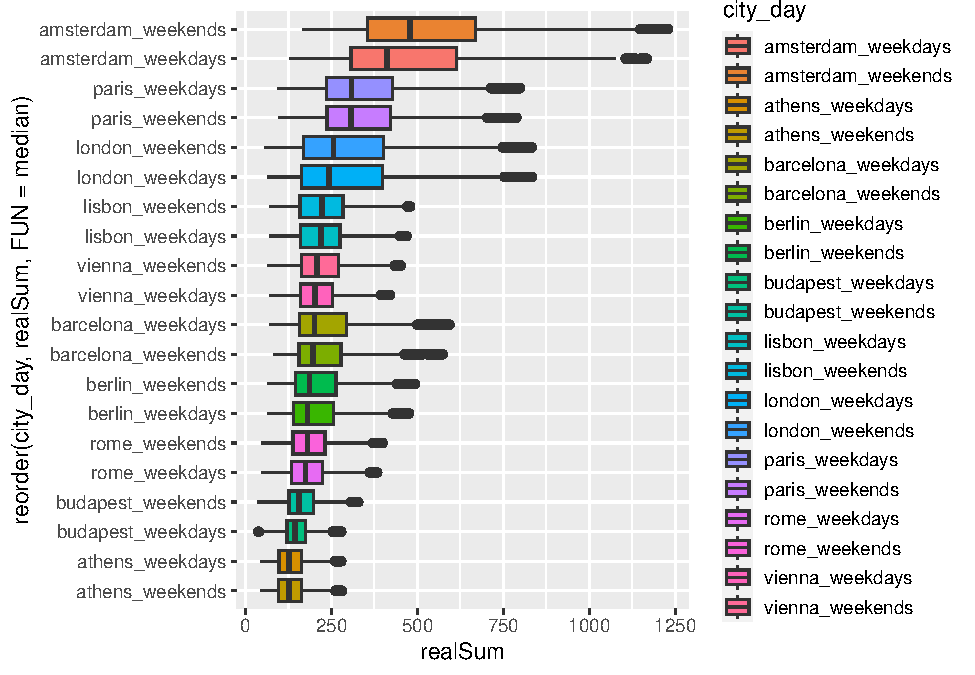
\includegraphics{Project_Prelim_report_files/figure-latex/unnamed-chunk-4-1.pdf}
The highest prices in europe are found in amsterdam.

\hypertarget{density-plot-of-price-vs-room-type}{%
\subsection{Density plot of Price vs Room
type}\label{density-plot-of-price-vs-room-type}}

\begin{Shaded}
\begin{Highlighting}[]
\FunctionTok{ggplot}\NormalTok{(my\_data, }\FunctionTok{aes}\NormalTok{(}\AttributeTok{x =}\NormalTok{ realSum, }\AttributeTok{group =}\NormalTok{ room\_type, }\AttributeTok{fill =}\NormalTok{ room\_type,}
    \AttributeTok{alpha =} \FloatTok{0.2}\NormalTok{)) }\SpecialCharTok{+} \FunctionTok{geom\_density}\NormalTok{()}
\end{Highlighting}
\end{Shaded}

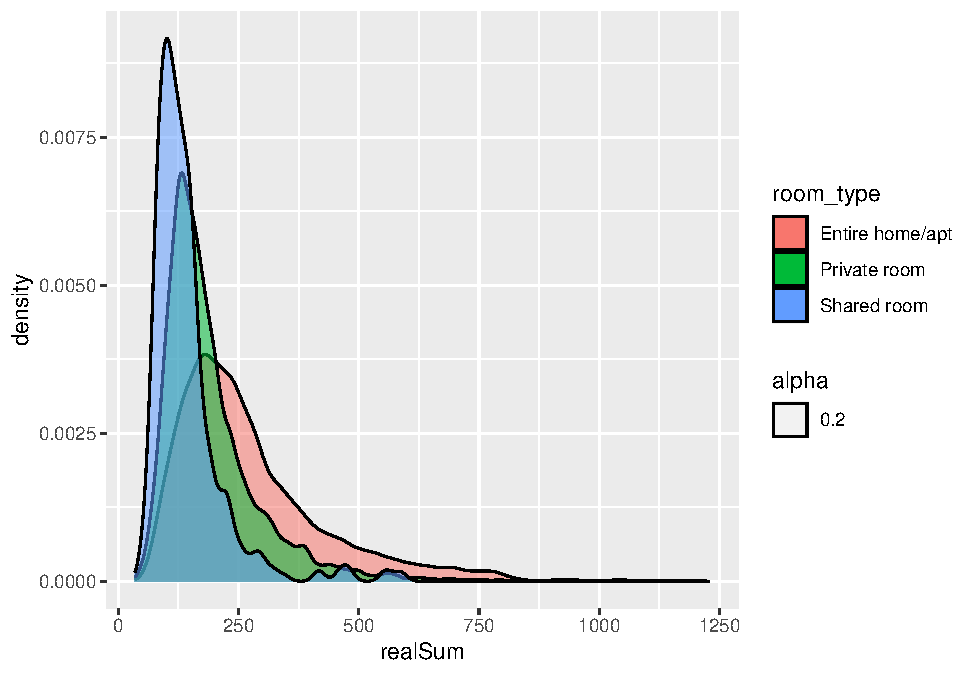
\includegraphics{Project_Prelim_report_files/figure-latex/unnamed-chunk-5-1.pdf}
The prices of entire home are high comparitively

\hypertarget{boxplot-of-city-vs-guest-satisfaction}{%
\subsection{Boxplot of City vs Guest
Satisfaction}\label{boxplot-of-city-vs-guest-satisfaction}}

\begin{Shaded}
\begin{Highlighting}[]
\FunctionTok{ggplot}\NormalTok{(my\_data, }\FunctionTok{aes}\NormalTok{(}\AttributeTok{x =} \FunctionTok{reorder}\NormalTok{(city\_day, guest\_satisfaction\_overall,}
    \AttributeTok{FUN =}\NormalTok{ median), }\AttributeTok{y =}\NormalTok{ guest\_satisfaction\_overall, }\AttributeTok{fill =}\NormalTok{ city\_day)) }\SpecialCharTok{+}
    \FunctionTok{geom\_boxplot}\NormalTok{() }\SpecialCharTok{+} \FunctionTok{coord\_flip}\NormalTok{() }\SpecialCharTok{+} \FunctionTok{theme}\NormalTok{(}\AttributeTok{legend.key.height =} \FunctionTok{unit}\NormalTok{(}\FloatTok{0.5}\NormalTok{,}
    \StringTok{"cm"}\NormalTok{), }\AttributeTok{legend.key.size =} \FunctionTok{unit}\NormalTok{(}\DecValTok{1}\NormalTok{, }\StringTok{"lines"}\NormalTok{))}
\end{Highlighting}
\end{Shaded}

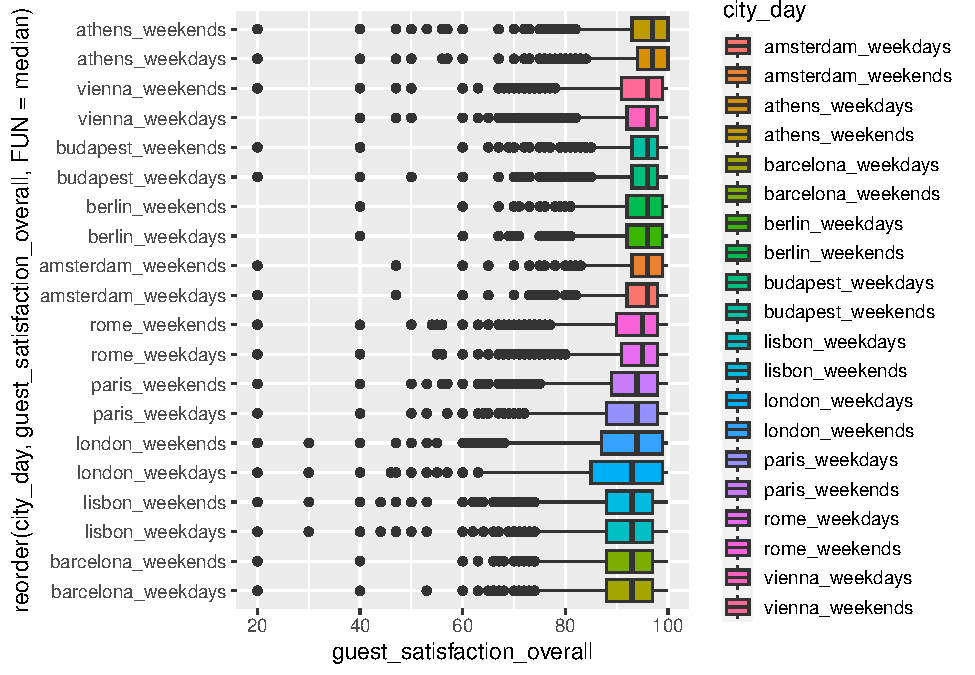
\includegraphics{Project_Prelim_report_files/figure-latex/unnamed-chunk-6-1.pdf}
This plot shows there is no major difference in Guest Satisfaction vs
City.

\hypertarget{scatterplot-of-price-vs-guest-satisfaction-filtered-by-city}{%
\subsection{Scatterplot of Price vs Guest Satisfaction filtered by
city}\label{scatterplot-of-price-vs-guest-satisfaction-filtered-by-city}}

\begin{Shaded}
\begin{Highlighting}[]
\FunctionTok{ggplot}\NormalTok{(my\_data, }\FunctionTok{aes}\NormalTok{(}\AttributeTok{x =}\NormalTok{ realSum, }\AttributeTok{y =}\NormalTok{ guest\_satisfaction\_overall,}
    \AttributeTok{color =}\NormalTok{ city\_day)) }\SpecialCharTok{+} \FunctionTok{geom\_point}\NormalTok{() }\SpecialCharTok{+} \FunctionTok{xlab}\NormalTok{(}\StringTok{"Price"}\NormalTok{) }\SpecialCharTok{+} \FunctionTok{ylab}\NormalTok{(}\StringTok{"Guest Satisfaction Overall"}\NormalTok{) }\SpecialCharTok{+}
    \FunctionTok{scale\_color\_discrete}\NormalTok{(}\AttributeTok{name =} \StringTok{"City{-}Day"}\NormalTok{)}
\end{Highlighting}
\end{Shaded}

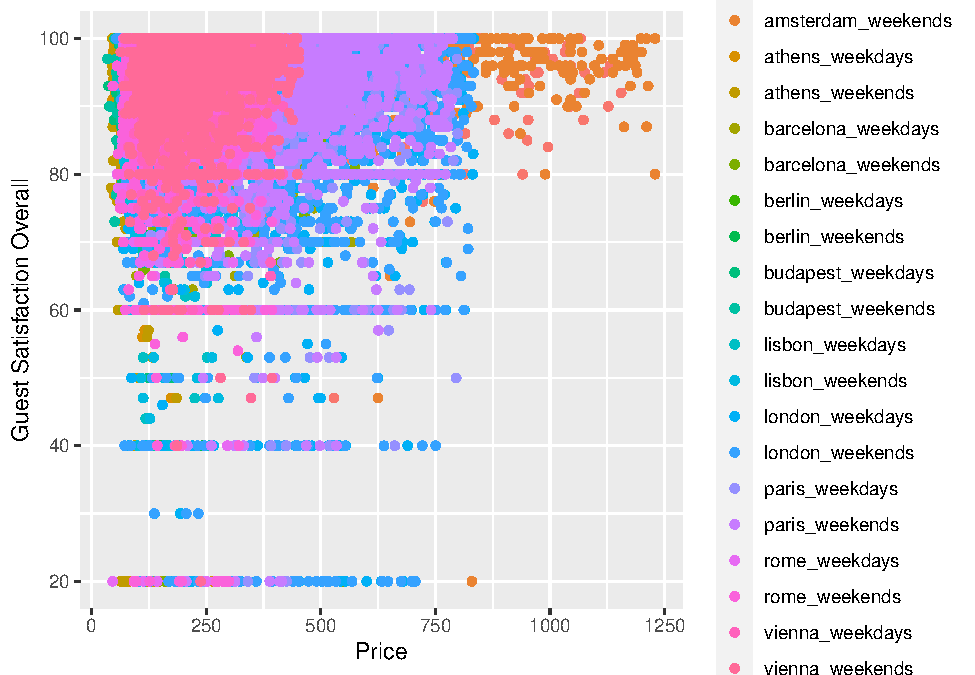
\includegraphics{Project_Prelim_report_files/figure-latex/unnamed-chunk-7-1.pdf}
This plot implies there are good cheaper Airbnb at most cities which
give higher guest satisfaction rating

\hypertarget{scatterplot-of-prices-in-rome-w.r.t-latitude-and-longitude-during-weekdays}{%
\subsection{Scatterplot of Prices in Rome w.r.t Latitude and Longitude
during
weekdays}\label{scatterplot-of-prices-in-rome-w.r.t-latitude-and-longitude-during-weekdays}}

\begin{Shaded}
\begin{Highlighting}[]
\NormalTok{tema }\OtherTok{\textless{}{-}} \FunctionTok{theme}\NormalTok{(}\AttributeTok{plot.title =} \FunctionTok{element\_text}\NormalTok{(}\AttributeTok{size =} \DecValTok{23}\NormalTok{, }\AttributeTok{hjust =} \FloatTok{0.5}\NormalTok{),}
    \AttributeTok{axis.text.x =} \FunctionTok{element\_text}\NormalTok{(}\AttributeTok{size =} \DecValTok{19}\NormalTok{, }\AttributeTok{face =} \StringTok{"bold"}\NormalTok{), }\AttributeTok{axis.text.y =} \FunctionTok{element\_text}\NormalTok{(}\AttributeTok{size =} \DecValTok{19}\NormalTok{,}
        \AttributeTok{face =} \StringTok{"bold"}\NormalTok{), }\AttributeTok{axis.title.x =} \FunctionTok{element\_text}\NormalTok{(}\AttributeTok{size =} \DecValTok{19}\NormalTok{),}
    \AttributeTok{axis.title.y =} \FunctionTok{element\_text}\NormalTok{(}\AttributeTok{size =} \DecValTok{19}\NormalTok{), }\AttributeTok{legend.text =} \FunctionTok{element\_text}\NormalTok{(}\AttributeTok{colour =} \StringTok{"black"}\NormalTok{,}
        \AttributeTok{size =} \DecValTok{19}\NormalTok{, }\AttributeTok{face =} \StringTok{"bold"}\NormalTok{), }\AttributeTok{legend.background =} \FunctionTok{element\_rect}\NormalTok{(}\AttributeTok{fill =} \StringTok{"\#F5FFFA"}\NormalTok{,}
        \AttributeTok{size =} \FloatTok{0.5}\NormalTok{, }\AttributeTok{linetype =} \StringTok{"dashed"}\NormalTok{, }\AttributeTok{colour =} \StringTok{"black"}\NormalTok{))}

\NormalTok{rome\_data }\OtherTok{\textless{}{-}}\NormalTok{ my\_data }\SpecialCharTok{\%\textgreater{}\%}
    \FunctionTok{subset}\NormalTok{(city\_day }\SpecialCharTok{==} \StringTok{"rome\_weekdays"}\NormalTok{)}

\FunctionTok{ggplot}\NormalTok{(}\AttributeTok{data =}\NormalTok{ rome\_data, }\AttributeTok{mapping =} \FunctionTok{aes}\NormalTok{(}\AttributeTok{x =}\NormalTok{ lat, }\AttributeTok{y =}\NormalTok{ lng)) }\SpecialCharTok{+} \FunctionTok{theme\_minimal}\NormalTok{() }\SpecialCharTok{+}
    \FunctionTok{scale\_fill\_identity}\NormalTok{() }\SpecialCharTok{+} \FunctionTok{geom\_point}\NormalTok{(}\AttributeTok{mapping =} \FunctionTok{aes}\NormalTok{(}\AttributeTok{color =}\NormalTok{ realSum),}
    \AttributeTok{size =} \DecValTok{3}\NormalTok{) }\SpecialCharTok{+} \FunctionTok{ggtitle}\NormalTok{(}\StringTok{""}\NormalTok{) }\SpecialCharTok{+}\NormalTok{ tema}
\end{Highlighting}
\end{Shaded}

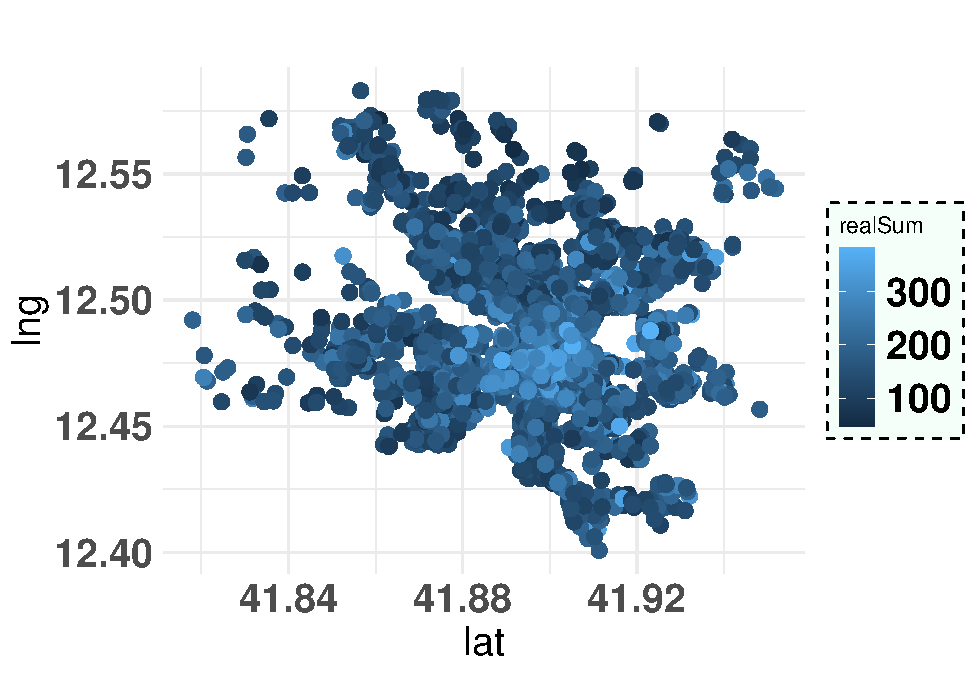
\includegraphics{Project_Prelim_report_files/figure-latex/unnamed-chunk-8-1.pdf}
This plot is within expectations of game theory, which suggests similar
types of establishments (price and hospitality) tend be in clusters.

\end{document}
